\chapter{Tides and Eclipses}

You live with a lot of orbital paths:
\begin{itemize}

\item The earth is spinning.  If you are standing at the equator,  you are traveling at 1,674 km per hour around the center of the planet.  We are all spinning east,  thus the sun comes up in the east and sets in the west.

\item  The earth is orbiting the sun.    It takes 365.242 days for the earth to go once around the sun.  This is why different constellations appear at different times during the year -- we only see the stars at night and the direction of night shifts as the earth moves around the sun.  

\item The moon is orbiting the earth.   The moon travels once around the earth once every 27.3 days.  

\end{itemize}

You can see the effects of these orbits on our planet.  Let's go over a few.

\section{Leap Years}

Note that it takes 365.242 days for the earth to go around the sun.  If we declared "The calendar will \emph{always} be 365 days per year!"  then gradually the seasons would shift by 0.242 days every year.  After a century,  they would have migrated 24 days.

So, we made a rule: "Every fourth year,  we will add an extra day to the calendar!"  The years 2021, 2022,and 2023 get no February 29th.  2024 gets a February 29th.

That got us a calendar with an average 365.25 days per year, so the seasons would not have migrated as quickly,  but they still would have migrated about three days every four hundred years.

So, we made another rule: "There will be no February 29th in the three century years (multiples of 100) that are not multiples of 400."  So the year 1900 had no Feb 29,  but the year 2000 had one.   Now the average number of days per year is 365.2425.


\section{Phases of the Moon}

The earth, the moon, and the sun form a triangle.   If you were standing on the moon,  you could measure the angle between the light coming from the sun and the the light going to the earth.   That angle would fluctuate between 0 degrees and 180 degrees.  
\begin{itemize}
\item When the angle was close to 0,  the people on earth would see a full moon.  
\item When the angle was close to 90 degrees,  the people on earth would see a half moon. 
\item When the angle was nearing 180 degrees, the people on earth would see a slim crescent.
\item When the angle was very close to 180 degrees,  the moon would be dark.  This is called a "new moon." 
\end{itemize}

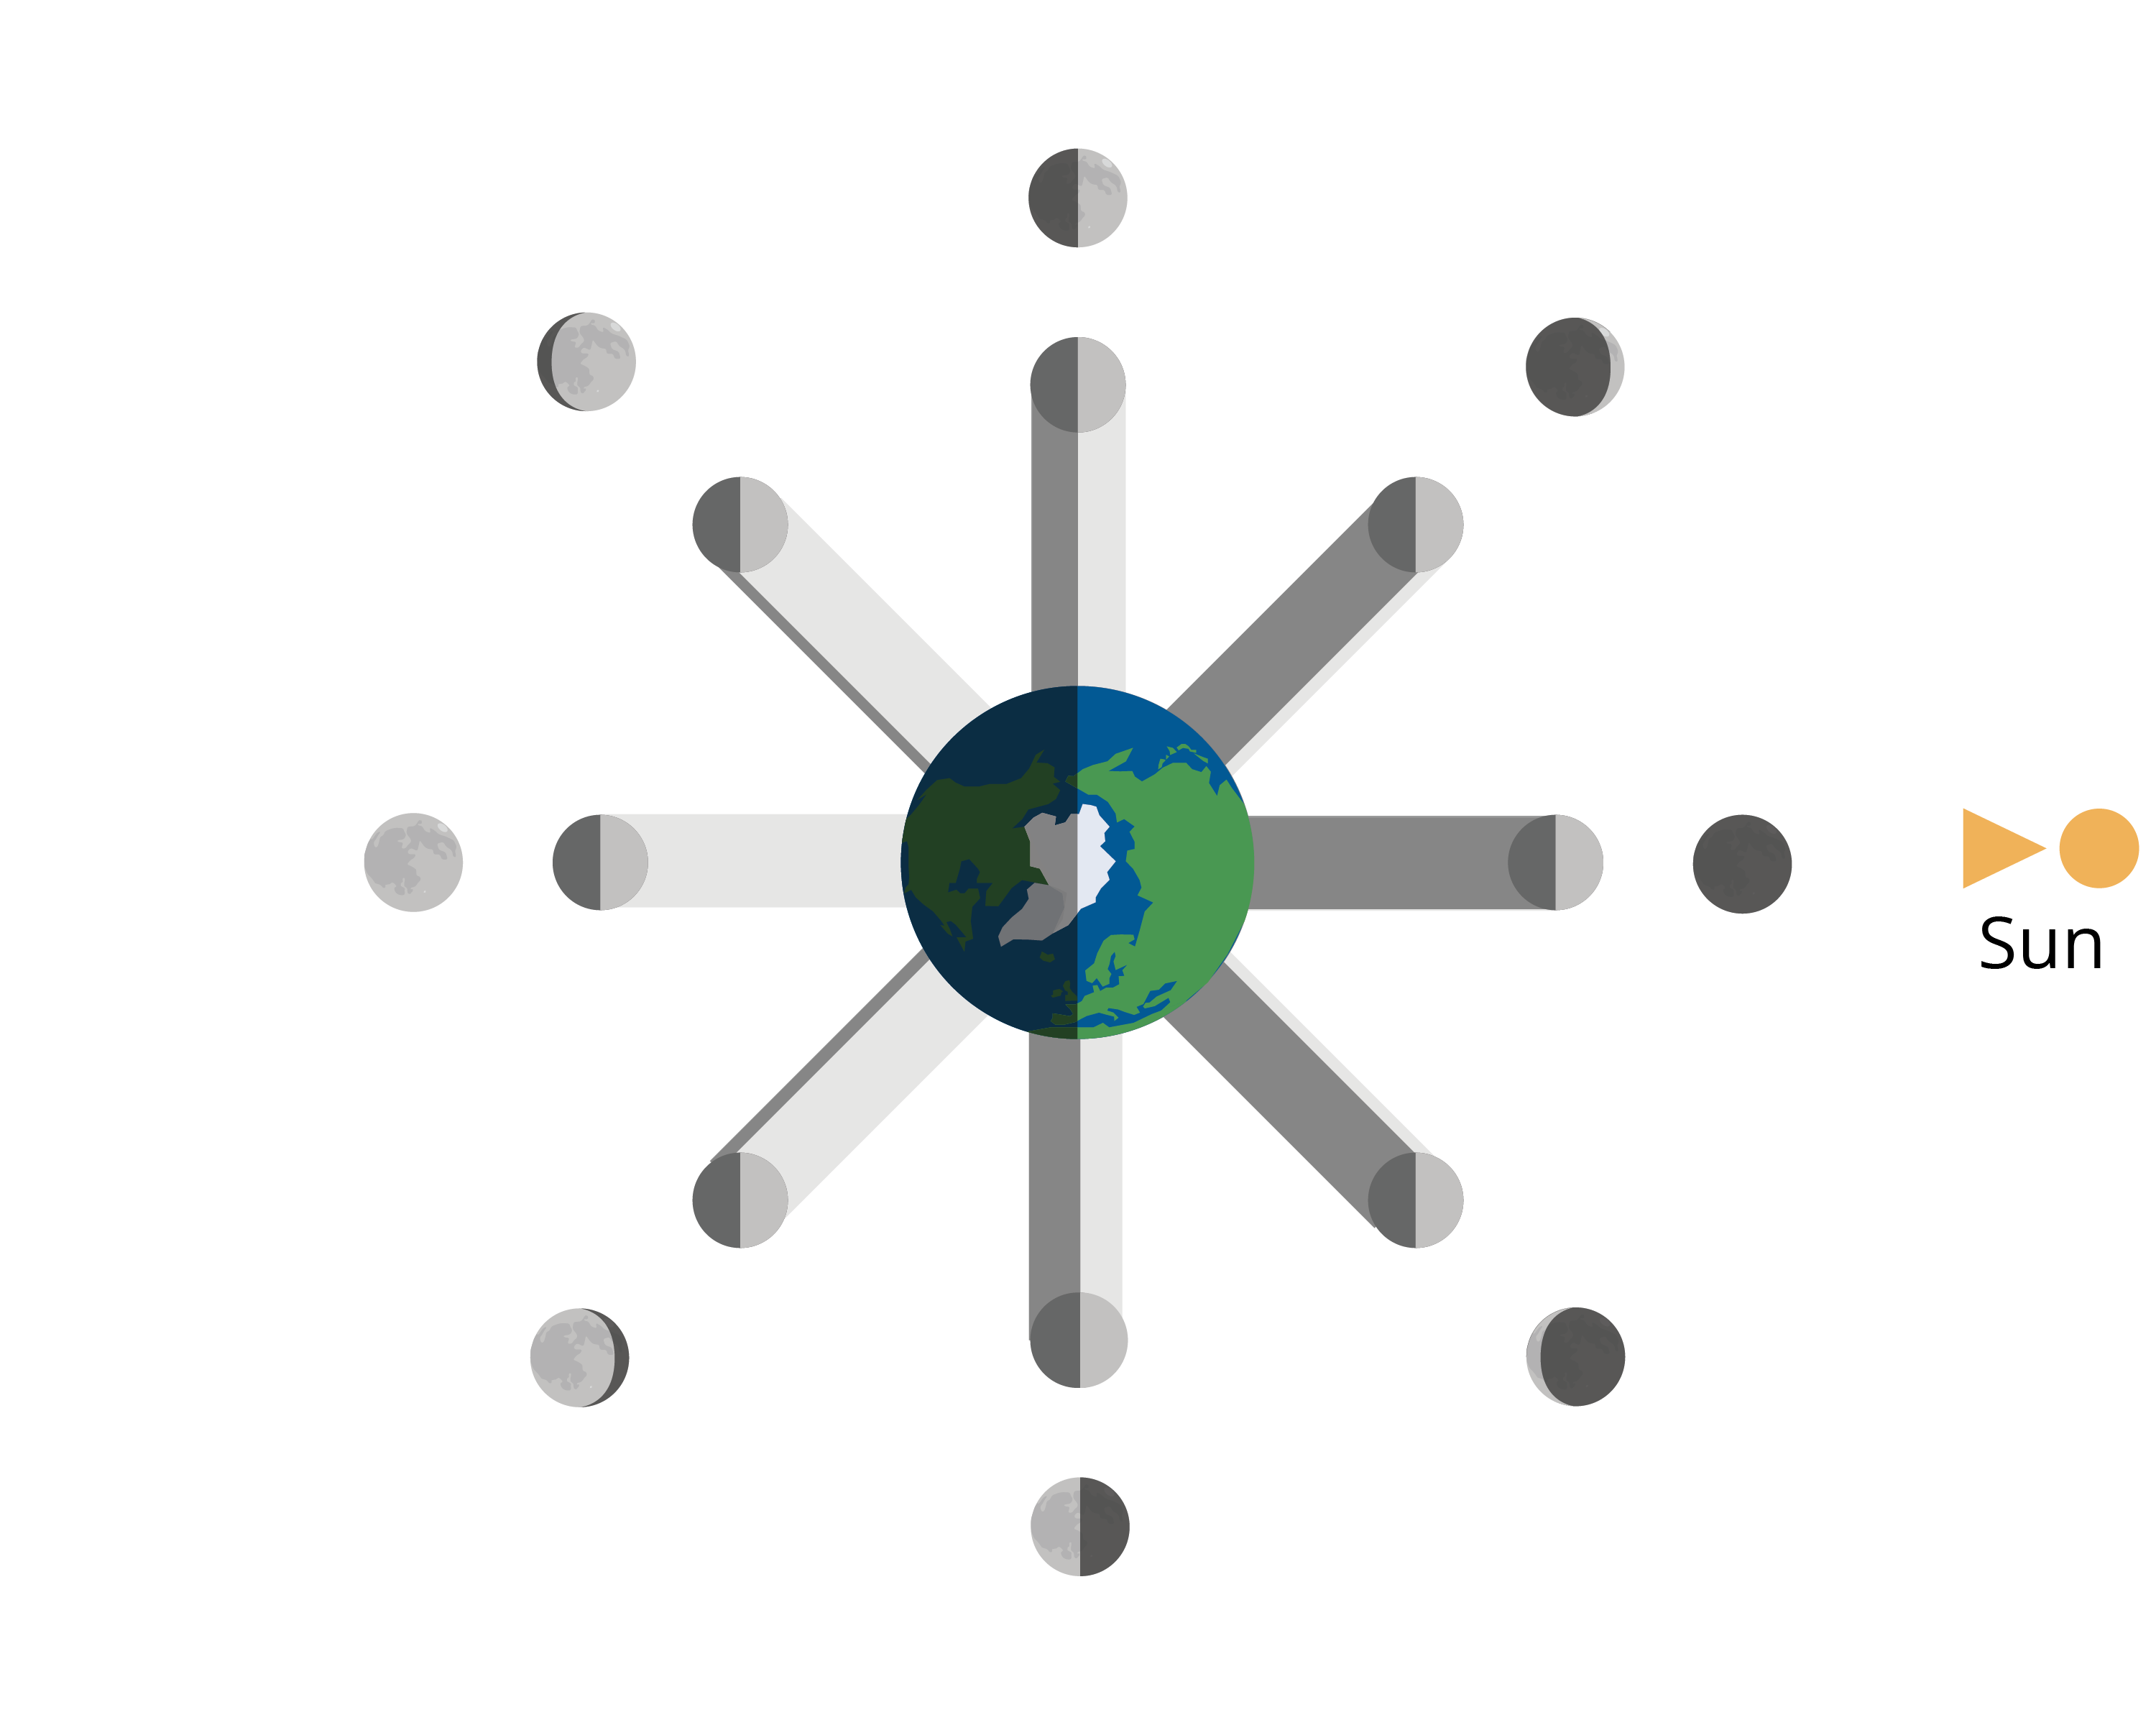
\includegraphics[width=.7\textwidth]{moonPhase.png}


Even though it takes 27.3 for the moon to travel around the earth once,   it takes 29.5 days to get from one full moon to the next. Why?  In the 27.3 days that it took the moon to travel around the earth,  the earth has moved about 17 degrees around the sun.  To get back into the same triangle configuration takes another 2.2 days.

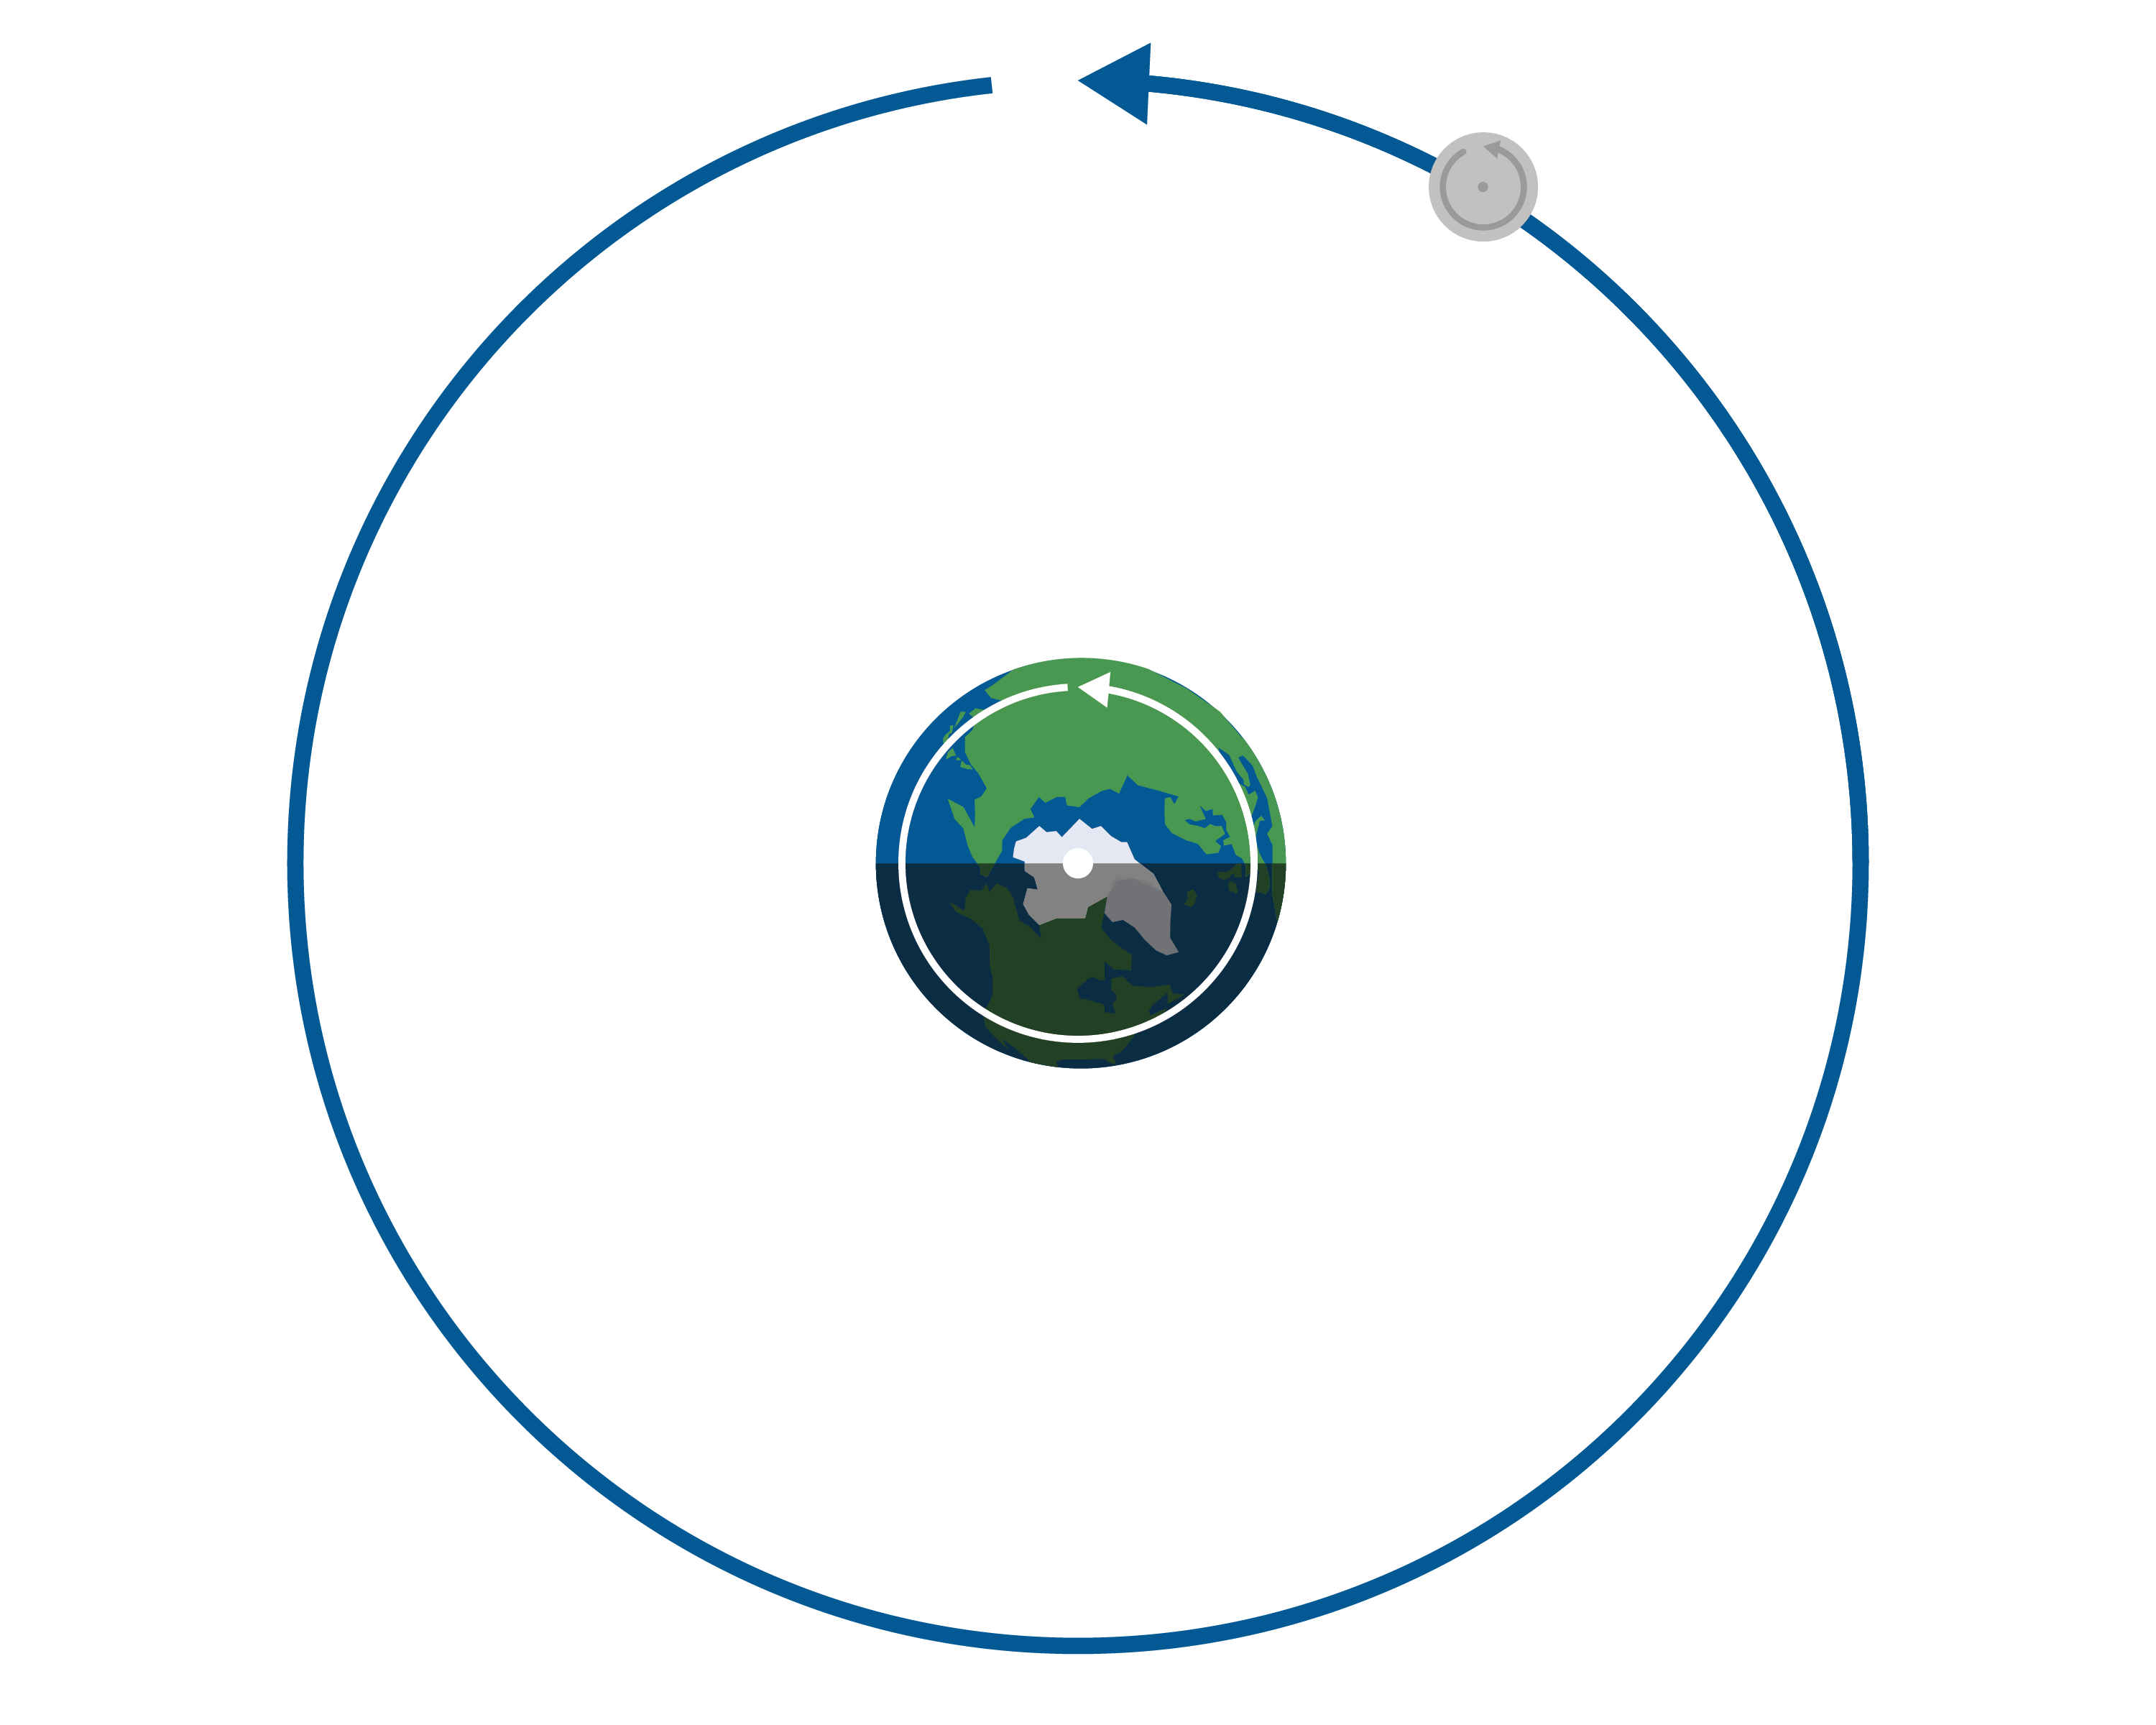
\includegraphics[width=.7\textwidth]{earthmoon.png}

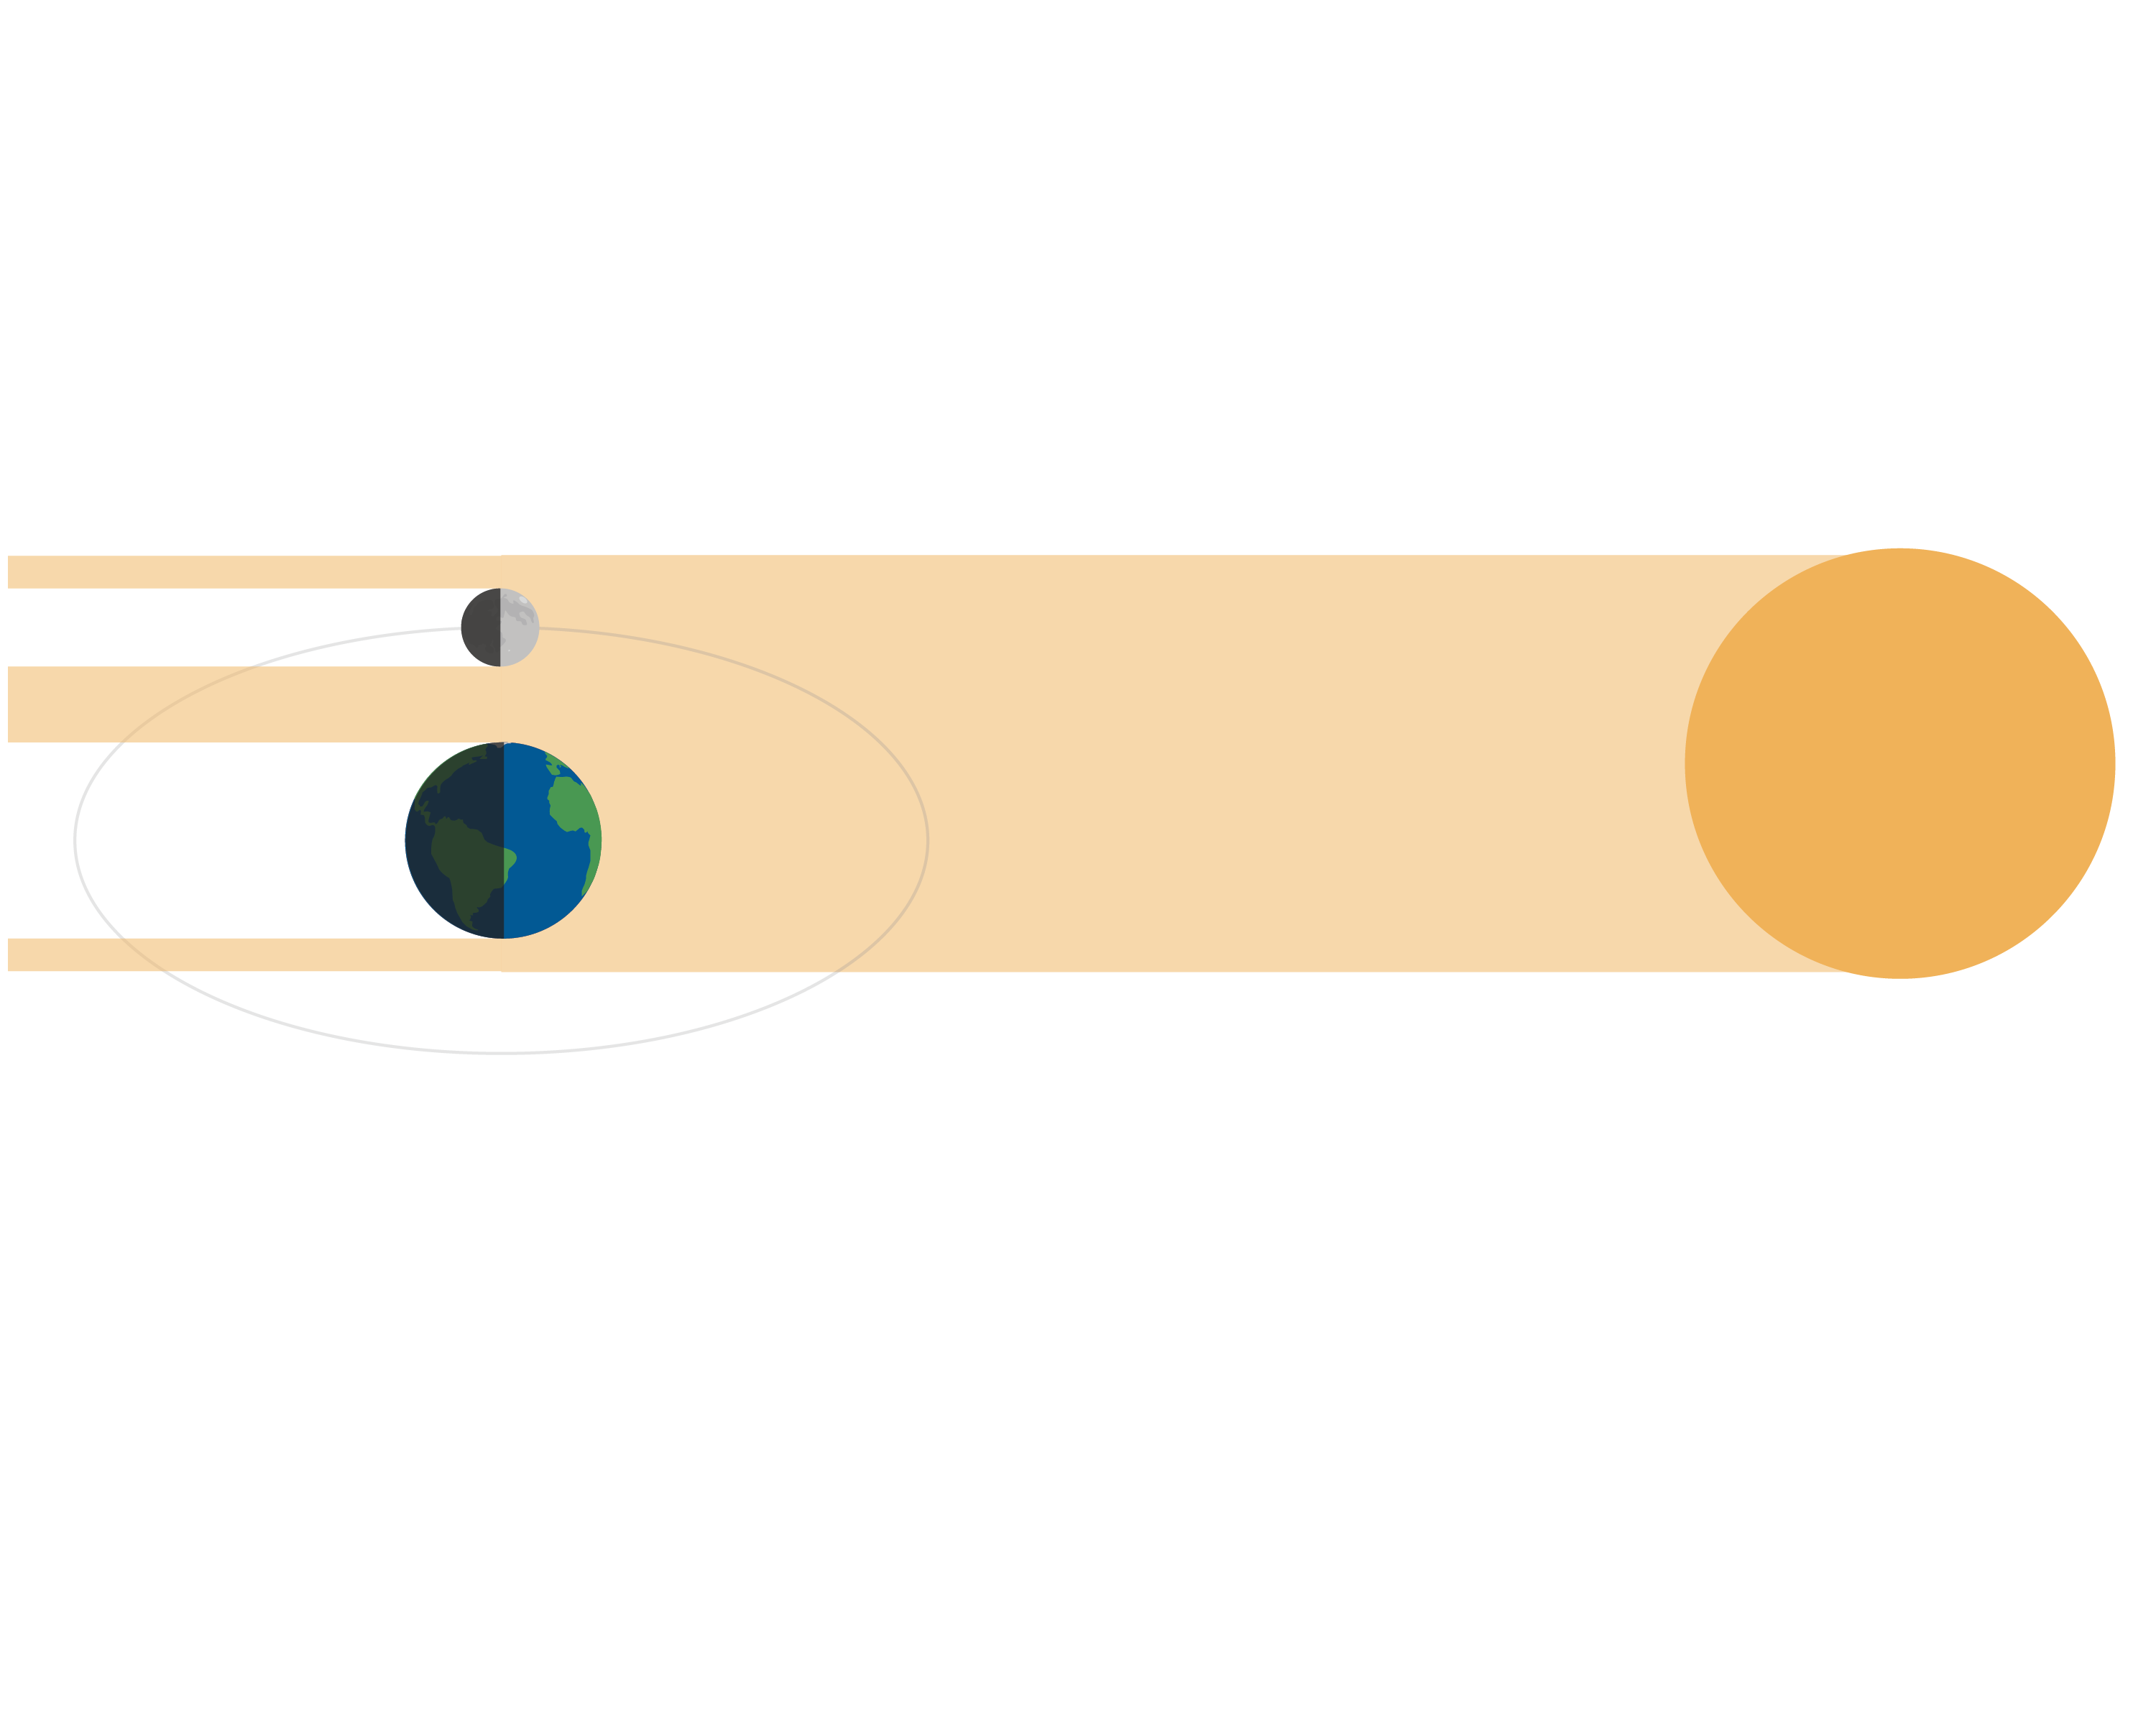
\includegraphics[width=.7\textwidth]{moonspace.png}


To explain why we often see a curve in the shadow of the moon, we can look at a ball that has one side painted yellow and the other red. 

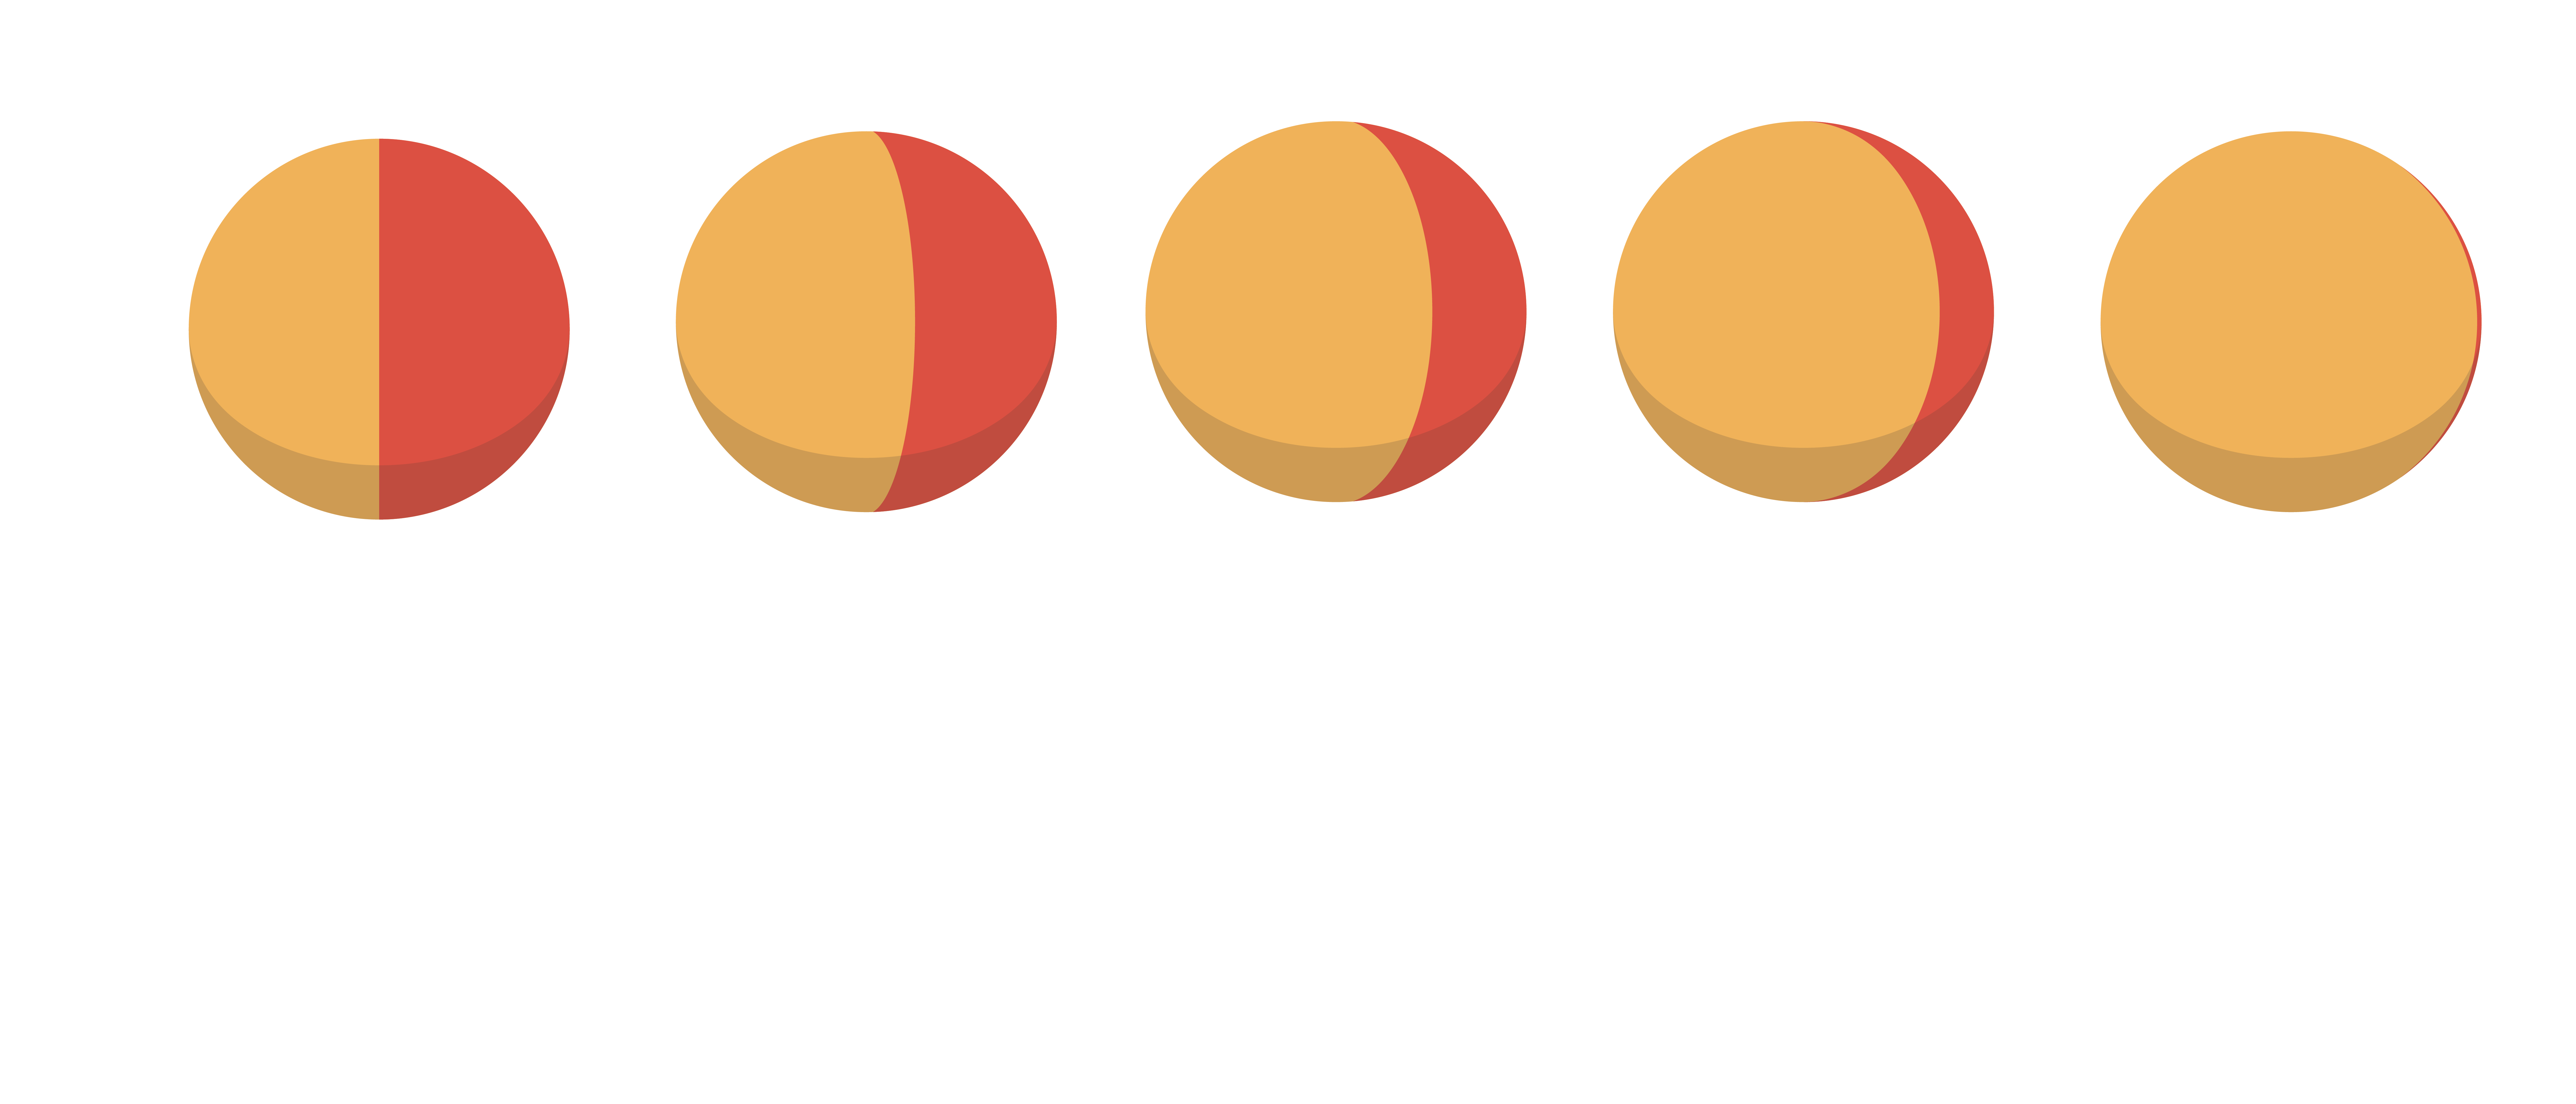
\includegraphics[width=.5\textwidth]{circleShading.png}

As we rotate the ball, we can see that the straight color boundary between each hemisphere begins to look curved. The curve we see in the moon is due to this same basic principle of how the shading of spheres works.    

FIXME: Add text about scale
In all of these graphics, we’ve been using incorrect scale. Here’s the true scale of the distance of the earth and the moon with accurate radii. 

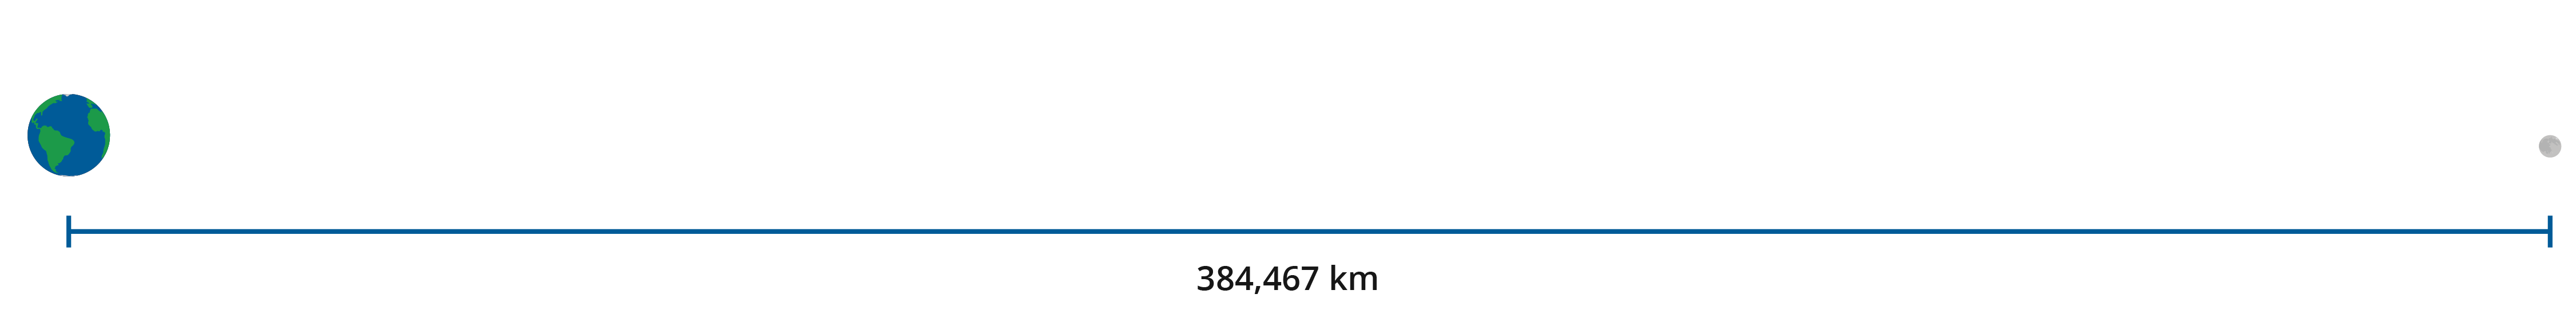
\includegraphics[width=.7\textwidth]{moonEarthScale.png}


FIXME: Add text about tidal lock


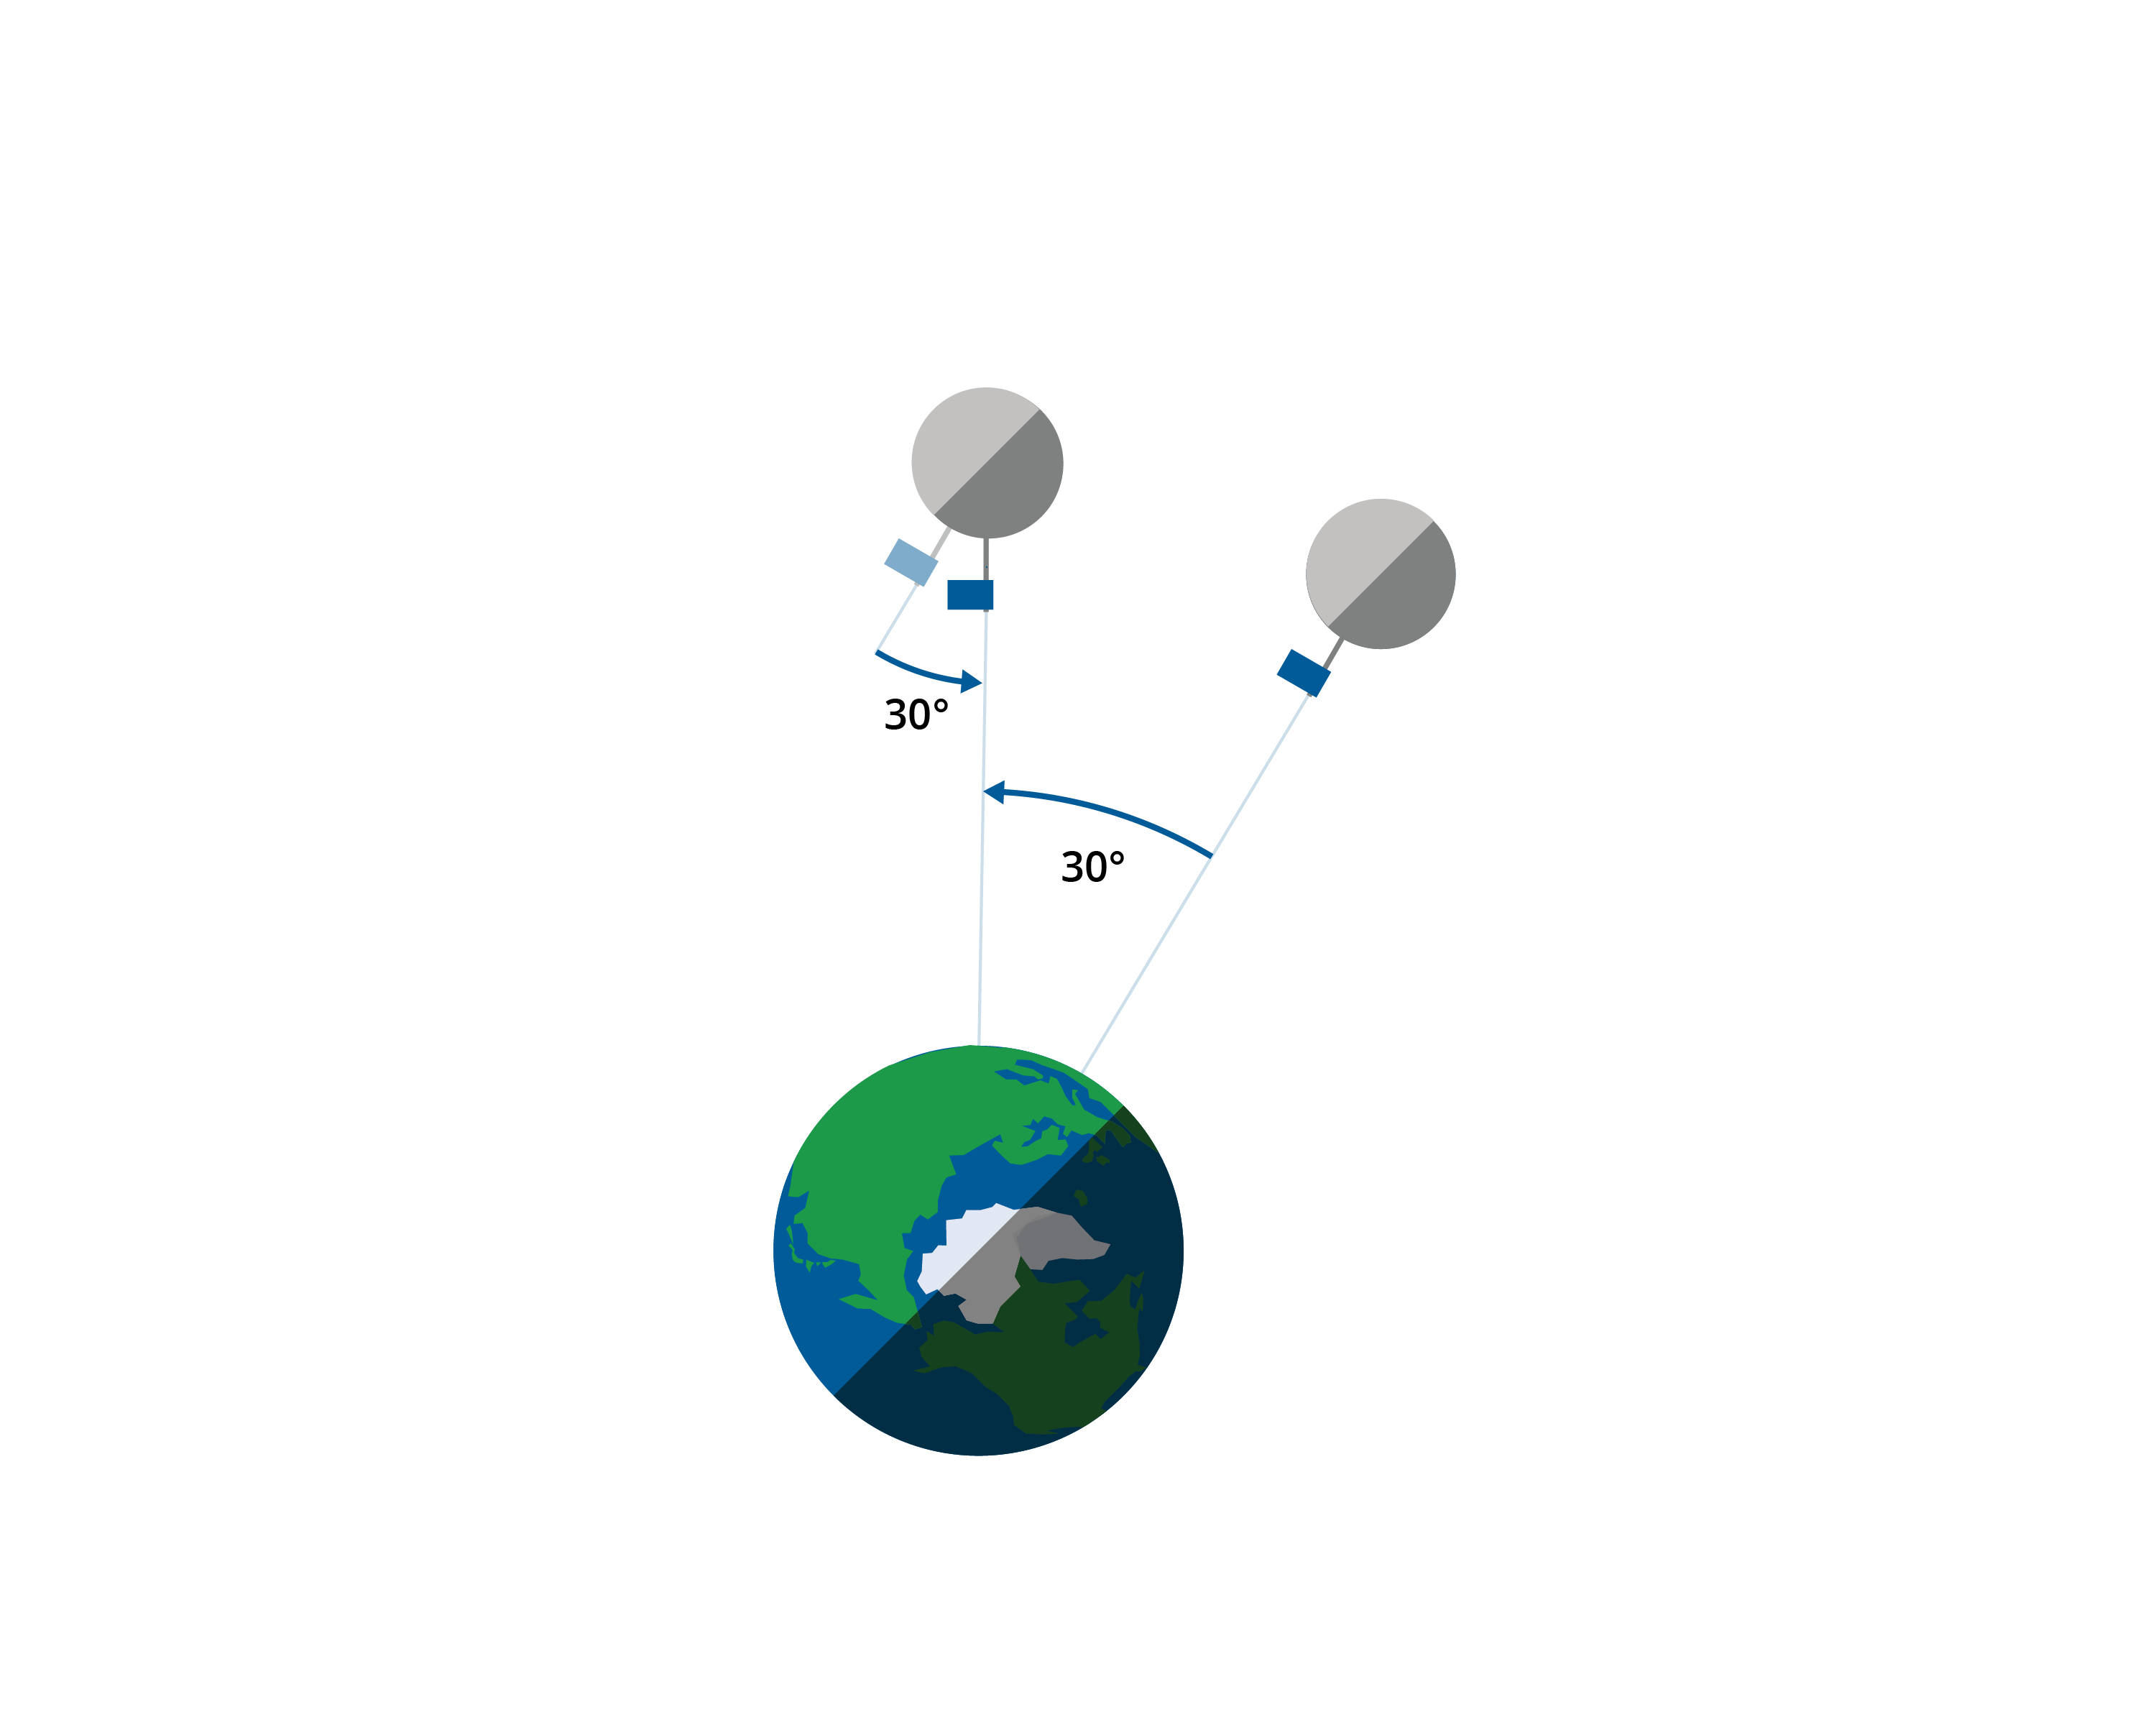
\includegraphics[width=.7\textwidth]{moonRotate.png}

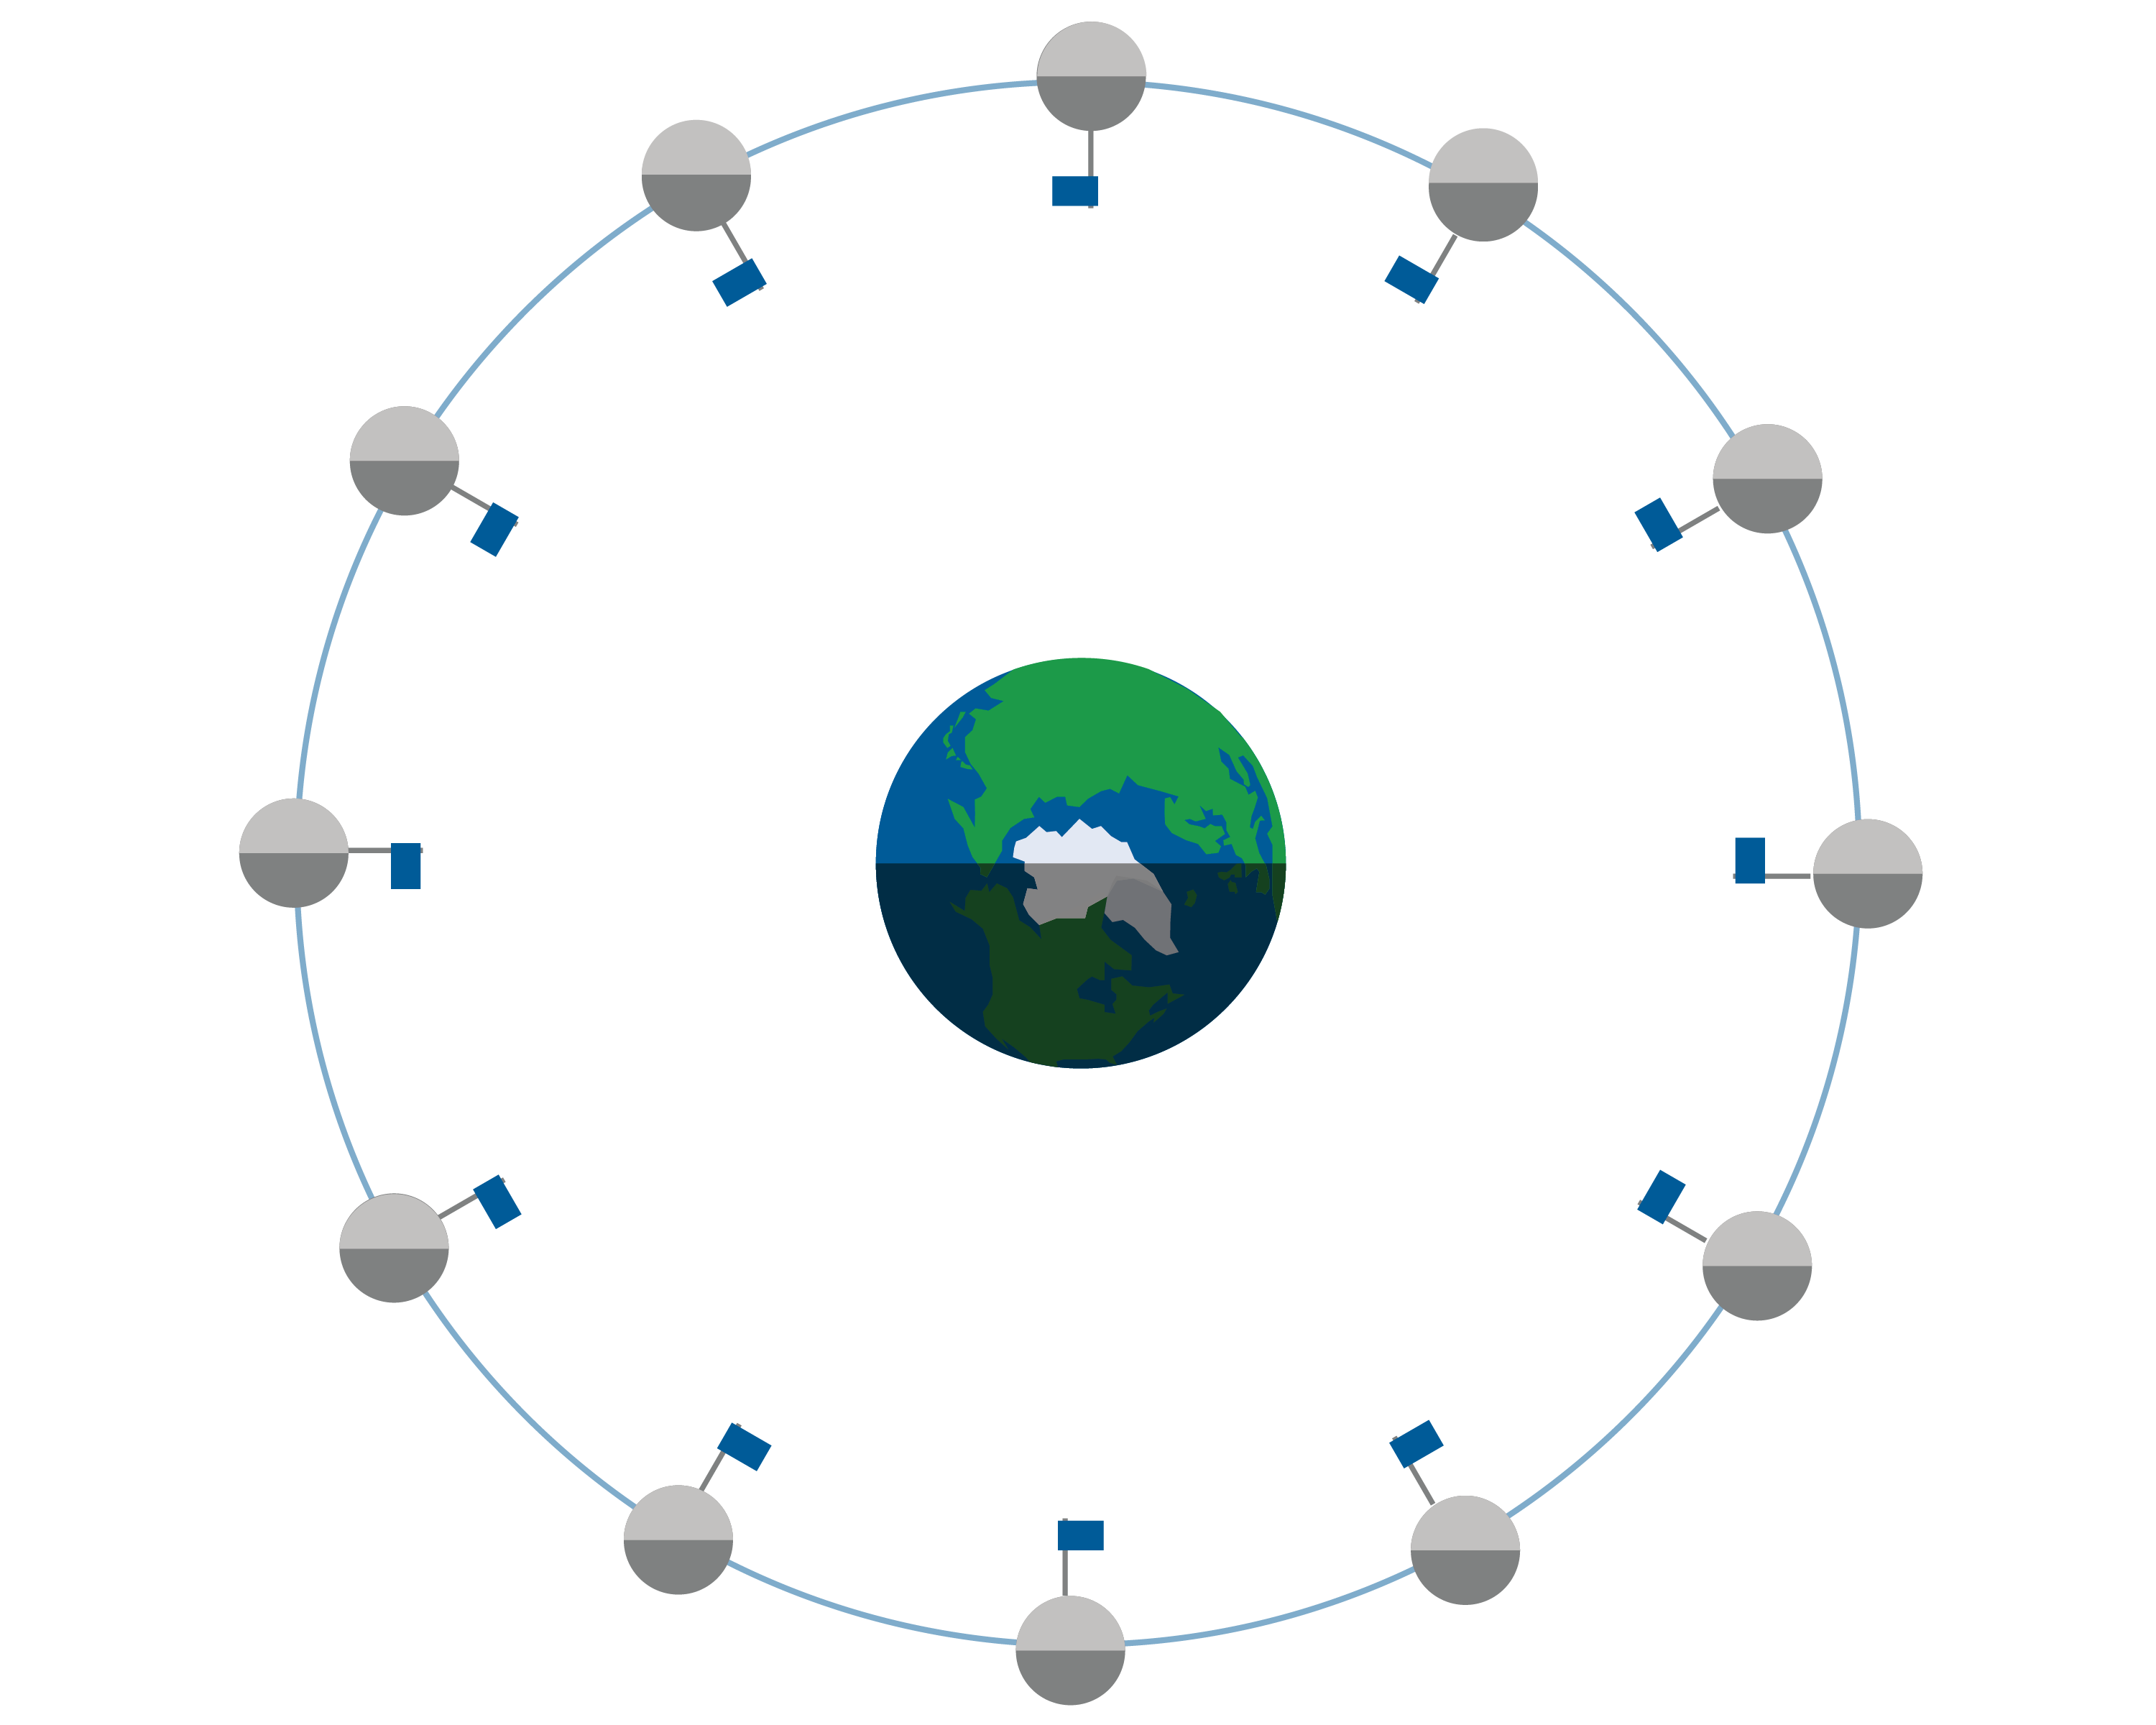
\includegraphics[width=.7\textwidth]{moonCircleRotate.png}



\section{Eclipses}

While the earth orbits the sun and the moon orbits the earth,  the two orbits are \emph{not in the same plane}.
We call the plane that the earth orbits the sun in the \newterm{ecliptic plane}.   The plane of the moon's orbit is about  5 degrees tilted from the ecliptic plane.

Note that the moon passes through the ecliptic plane only twice every 27.3 days.   Imagine that at the instant it passed through the ecliptic plane was also the precise instant of a full moon.    The sun, the earth, and the moon would be in a straight line!  The earth would cast a shadow upon the moon -- it would go from a bright full moon to a dark moon until the moon moved back out of the shadow of the earth.   This is known as a \newterm{lunar eclipse}.

The diameter of the moon is a little more than a quarter the diameter of the earth,  so they don't have to be in perfect alignment for the moon to be darkened.   Lunar eclipses actually happen once or twice per year.

Now imagine that at the instant the moon passed through the ecliptic plane was also the precise instant of a new moon.    The sun,  the moon, and the earth would be in a straight line!  The moon would cast a shadow upon some part of the earth.  To a person in that shadow,  the sun disappear behind the moon.   This is known as a \newterm{solar eclipse}.

The sun is pretty big,  so if the moon blots out just part of it,  we call it a \newterm{partial solar eclipse}.  There are a few partial solar eclipses every year.   Note that because the moon's shadow is too small to shade the whole earth,   only certain parts of the world will experience any solar eclipses. 

Every 18 months or so,  there is a total eclipse of the sun.  Once again,  only certain parts of the world experience it.   You can expect to experience a total eclipse of the sun at your home about once every 375 years.
 
\section{The Far Side of the Moon}

Like the earth,  the moon spins on its axis.  Due to earth's gravity,  the rotation of the moon slowed down until its spin matched the rate it orbits earth.  That is: we are always looking at the same side of the moon.  Until we orbited the moon,  we had no idea what the far side looked like.

Some people call it "The Dark Side of the Moon," but it gets just as much sunshine as the side that faces earth.  The name comes from the fact that we lose communication with spacecraft (like the Apollo missions to the moon) when they are on the far side of the moon.  When we lose communications with a craft, 
we often say "It went dark."

\section{Tides}

When we say "The moon orbits the earth,"  that is a bit of an oversimplification.  The force of gravity that pulls the moon toward the earth,  also pulls the earth toward the moon.   The earth is about 81 times heavier
than the moon,  so the moon moves more, but the moon definitely moves the earth.

The center of the moon and the center of the rotate around each other.  The point they rotate around is inside the the earth,  but it is closer to the surface of the earth than it is to the center of the earth.

Orbits happen, remember, when the centripetal force is equal to gravitational force.  So the centripetal force created by the earth being swung by the moon is equal to the gravitational force that the moon exerts on all the mass on the moon.

However.  

The parts of the earth that are closer to the moon experience less centripetal force (away from the moon) and more gravitational force (toward the moon).

The parts of the earth that are farther from the moon experience more centripetal force (away from the moon) and less gravitational force (away from the moon).   

The effects are not big.  For example,  you won't notice that you can jump higher when the moon is 
overhead.  You will lose only about 1/200,000 of your weight.

But the ocean is huge.: 1/200,000 of its weight is a lot of force.

The water in the oceans bulges a little both toward the moon and away from it.

The earth is still rotating.  If you are at the beach as your longitude slides into one of these bulges,   you say "Hey, the tide is rising!"  The peak of these bulges is known as "high tide".  Because there is a bulge on each 
side of the planet,  high tide comes twice a day.

This is a lunar tide -- because it is caused by the moon.  There is a similar effect from the sun,  but the sun is very, very far away: solar tidal forces are about half as powerful lunar tidal forces.  When the sun and the moon work together,   the tides are stronger.  This is called a \newterm{spring tide}.   Spring tides don't happen in the spring time;  they happen close to full moons and new moons.

When the moon and the sun are working against each other,  the tides are weaker.  This is called a \newterm{neap tide}.  Neap tides happen when you see a half moon in the sky.

\subsection{Computing the Forces}

We are enumerating several forces that shape the water on the planet.  All these forces are pulling on your
body too.  In these exercises, you are going to calculate how each force would effect a 1 kg mass on the surface of the earth.

Here are some numbers you will need:
\begin{itemize}
\item The mass of the earth: $5.97219 \times 10^{24}$ kg
\item The mass of the sun:  $1.9891 \times 10^{30}$ kg
\item The mass of the moon: $7.347673 \times 10^{22}$ kg
\item Radius of the earth at the equator: $6,371$ km
\item Average distance from the center of the earth to the center of the sun:  $149.6 \times 10^6$ km
\item Average distance from the center of the moon to the center of the earth: $384,467$ km.
\end{itemize}


\begin{Exercise}[title={Life Among the Orbits 1: Earth Gravity}, label=life-orbits1]


If the earth were still and alone in the universe,  there would still be the force of gravity.  We have said that that a kilogram on the surface of the earth is pulled toward the center of the earth with a force of 9.8 N.   

\textbf{Confirm that the gravity of the earth pulls a 1kg mass on the surface of the planet with a force of about 9.8 N.}

You will need the formula for gravitation: 

$$F_g = \frac{g m_1 m_2}{r^2}$$

If we measure distance in km and mass in kg,  the gravitation constant $g$ is $6.67430 \times 10^{-17}$.  

\end{Exercise}
\begin{Answer}[ref=life-orbits1]

The earth and 1 kg on the surface would attract each other with a force of:

$$F_g = \frac{\left( 6.67430 \times 10^{-17} \right) \left(5.97219 \times 10^{24}\right) \left(1\right)}{6,371^2} =  
\frac{3.98583 \times 10^{8}}{4.0590 \times 10^{7}}  = 9.7987 \text{ N}$$

Thus, if the earth were still and alone in the universe,  the oceans would form a perfect sphere.

\end{Answer}

\begin{Exercise}[title={Life Among the Orbits 2: Earth Centripetal Force}, label=life-orbits2]

What if we add the spinning of the earth?  The spinning would try to throw the kg into space.  The 
formula for centripetal force is

$$F_c = \frac{m v^2}{r} $$

\textbf{Calculate the centripetal force on a 1 kg mass on the surface of the earth.   It doesn't fly off into space,  so the force due to gravity must be bigger.  How many times bigger?}

Assume that the mass is on the equator,  thus rotating around the earth at 465 m/s.

\textbf{Does the centripetal force increase, decrease, or stay the same as you get closer to the north pole?}

\end{Exercise}

\begin{Answer}[ref=life-orbits2]

$$F_c = \frac{(1) (465)^2}{6,371,000}  = 0.03373 \text{ N}$$

So the spinning of the earth is trying to throw you into space,  but the force of gravity is about 289 times more powerful.

This centripetal force decreases as you move from the equator to the north pole.   In fact, at the north pole, 
there is no centripetal force.   Thus, the spinning of the earth makes the oceans an oblate ellipsoid instead of a perfect sphere: the diameter going from pole-to-pole is shorter than a diameter measured at the equator.

You should feel a teensy-tiny bit lighter on your feet at the equator than you do at the north pole: 0.34\% lighter.

\end{Answer}

\begin{Exercise}[title={Life Among the Orbits 3: The Moon's Gravity}, label=life-orbits3]

Now we add the moon's gravitational force to our model.

When the moon is directly overhead,   how strongly will it pull at the 1 kg mass on the equator?

When the moon is directly underfoot,  how strongly will it pull at the 1 kg mass on the equator?

Is that a big difference?

\end{Exercise}

\begin{Answer}[ref=life-orbits3]

Overhead, the moon is $384,467 - 6,371 = 378,096$ km from your 1 kg mass.

$$F_g =  \frac{g m_1 m_2}{r^2} = \frac{\left( 6.67430 \times 10^{-17} \right) \left( 7.347673 \times 10^{22} \right) \left(1\right)}{378,096^2} =  
\frac{4.9040574 \times 10^{6}}{1.42956585216 \times 10^{11}}  = 3.43058 \times 10^{-5} \text{ N}$$

This is a very small force: The force due to earth's gravity is nearly three hundred thousand times stronger.

Underfoot, the moon is $384,467 + 6,371 = 390,838$

$$F_g =  \frac{g m_1 m_2}{r^2} = \frac{\left( 6.67430 \times 10^{-17} \right) \left( 7.347673 \times 10^{22} \right) \left(1\right)}{390,838^2} =  \frac{4.9040574 \times 10^{6}}{1.52754 \times 10^{11}} =  3.2103 \times 10^{-5} \text{ N}$$

The force due to the moon's gravity is about 6\% stronger when the the moon is overhead than when it is underfoot. 

\end{Answer}

\begin{Exercise}[title={Life Among the Orbits 4: The Swing of the Moon}, label=life-orbits4]

Now we add the moon's motion.  The moon and the earth swing each other around.  This creates a centripetal force.  They both travel in nearly a circle centered at their center of mass.

\textbf{How far is the center of mass of the moon and the earth from the center of the earth?}  (You can imagine a see-saw with the center of the earth on one end and the center of the moon on the other.   Where would the balance point be?)

\textbf{What point on the surface of the earth is closest to the center of mass?  How far is it?}

\textbf{What point on the surface of the earth is farthest from the center of mass?  How far is it?}


\end{Exercise}

\begin{Answer}[ref=life-orbits4]

If we let $r$ be the distance (in km) from the center of the earth to the center of mass,  the distance from
the center of the mass to the center of the moon is $384,467 - r$.

To find the balance point,  multiply each mass by how far it is from the center of mass:

$$\left( 5.97219 \times 10^{24} \right) r = \left( 7.347673 \times 10^{22} \right) \left(384,467 - r\right)$$

Solving for $r$:

$$ r = \frac{4,730.15}{1 + 0.0123} = 4,673 \text{ km} $$

The point on the earth closest to this?  It is where the moon is directly overhead.  The it is $6,371 - 4,673 = 1,698$ km from the center of mass.

The point on the earth farthest from this?  It is where the moon is directly underfoot.  The it is $6,371 + 4,673 = 11,044$ km from the center of mass.

\end{Answer}

\begin{Exercise}[title={Life Among the Orbits 5: Lunar Centripetal Force}, label=life-orbits5]

The moon swings us around that center of mass once every 27.3 days.  (Forget about the spinning of the earth for this part. )  What is the largest and smallest centripetal forces on the surface of the earth created by this swinging

What is the largest centripetal force on a 1 kg mass with the moon directly underfoot? (You need an answer from the previous question: There is a point on the surface of the earth that is 11,044,000 m from the center of gravity.)

What is the resulting centripetal force
on a 1 kg mass with the moon directly overhead?  (You will need the other answer from the previous exercise: That point is 1,698,000 m from the center of mass of the moon and the earth.)

For this problem is probably easier to use this formula for centripetal force:

$$F_c = m r \omega^2$$

Where $m$ is mass in kg,  $r$ is radius in m,  and $\omega$ is the angular velocity in radians per second.

\end{Exercise}

\begin{Answer}[ref=life-orbits5]

First,  lets figure out $\omega$.   It travels through $2\pi$ radians in 27.3 days.  27.3 days = 2,358,720 seconds.    $\omega = \frac{2\pi}{2,358,720} = 2.663811435 \times 10^{-6}$

$$F_c = (1)(11,044,000)(2.663811435 \times 10^{-6})^2 = 7.8365 \times 10^{-5}$$

Now the weakest:

$$F_c = (1)(1,698,000)(2.663811435 \times 10^{-6})^2 = 1.20512 \times 10^{-5}$$

\end{Answer}


\begin{Exercise}[title={Life Among the Orbits 6: Net  Force}, label=life-orbits6]

Now add together the two forces at both the nearest point to the moon and the farthest.

\end{Exercise}

\begin{Answer}[ref=life-orbits6]

Closest to the moon,   the gravitational force of the moon and the centripetal forces are in the same direction: toward the moon.

$$F_{total} = 1.20488 \times 10^{-5} + 3.43045 \times 10^{-5} = 4.6356 \times 10^{-5} \text{ N}$$

Farthest from the moon,  the gravitational force of the moon and the centripetal forces are in opposite directions:

$$F_{total} = 7.8367 \times 10^{-5} - 3.2104 \times 10^{-5} = 4.62604 \time 10^{-5} \text{N}$$

This is great conclusion:  The two forces are basically equal: one pulls the water closest to the moon toward the moon,  the other pulls water farthest from the moon away from the moon.

Both forces are pretty small:  The force due to earth's gravity is about $211,000$ times more than either.

And that is why there are two basically equally large high tides every day.

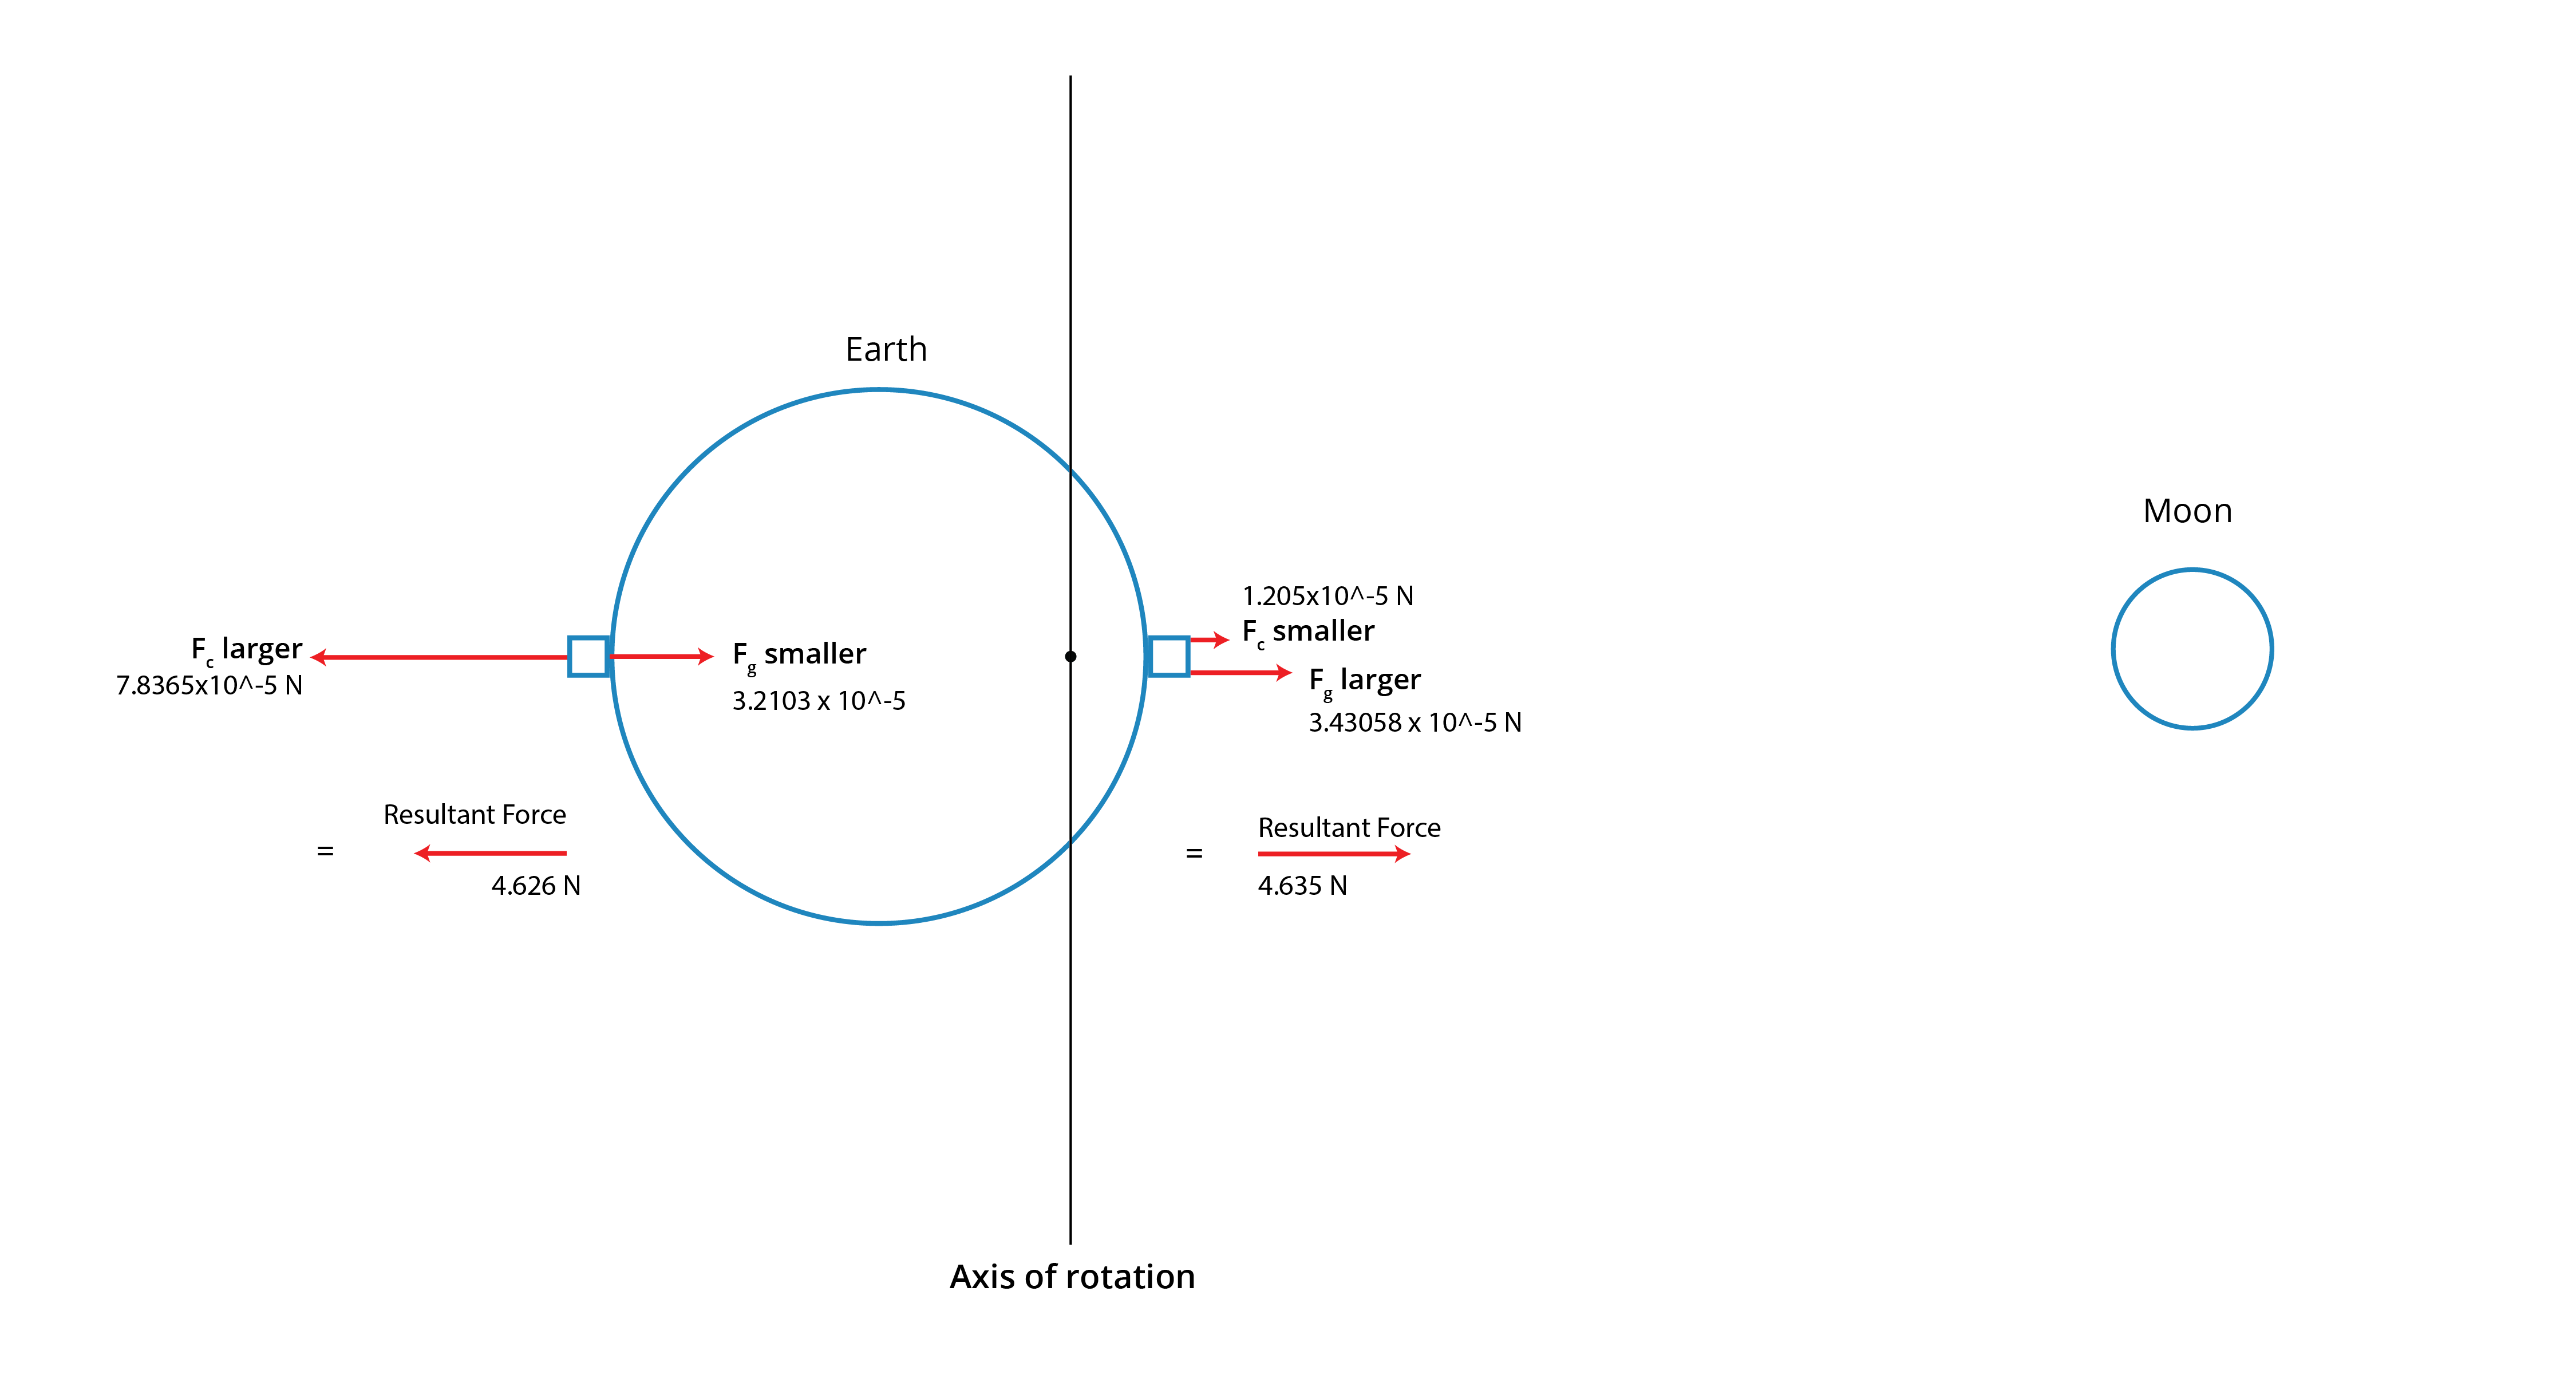
\includegraphics[width=.5\textwidth]{tidesSolution.png}

\end{Answer}


\subsection{Solar Tidal Forces}

The sun has a much larger gravitational effect on the earth than the moon does:
\begin{itemize}
\item When the sun is overhead,  it will pull on a 1 kg mass with a force of about 0.00593 N.
\item When the moon is overhead,  it will pull on a 1 kg mass with a force of about 0.0000343 N.
\end{itemize}

Why are lunar tides about twice as powerful solar tides?

Tides occur because the pull of gravity and the pull of the centripetal force are out of balance somewhere on the planet.  The sun is so far away that the effects of gravitational and centripetal forces are very close to equal everywhere on earth.





